%%%%%%%%%%%%%%%%%%%%%%%%%%%%%%%%%%%%%%%%%%%%%%%%%%%%
% Overview
%%%%%%%%%%%%%%%%%%%%%%%%%%%%%%%%%%%%%%%%%%%%%%%%%%%%
\section{Independent Particle Shell Model}
A nucleus is a tiny object with its typical size of about 1.2~fm, which, however, is a complicated many-body system where nucleons are bound by strong interactions. To fully understand the detailed structure of the nucleus, one needs to have the complete knowledge of each nucleons' eigen-state. For a light nucleus with only few nucleons, the wave functions can be directly calculated using variational methods~\cite{PhysRevLett.87.172502}. However, for medium and heavy nuclei ($A\geq 12$), the explosion of degree of freedom in the Hamiltonian makes it impossible to obtain the solution.
\begin{figure}[!ht]
  \begin{center}
    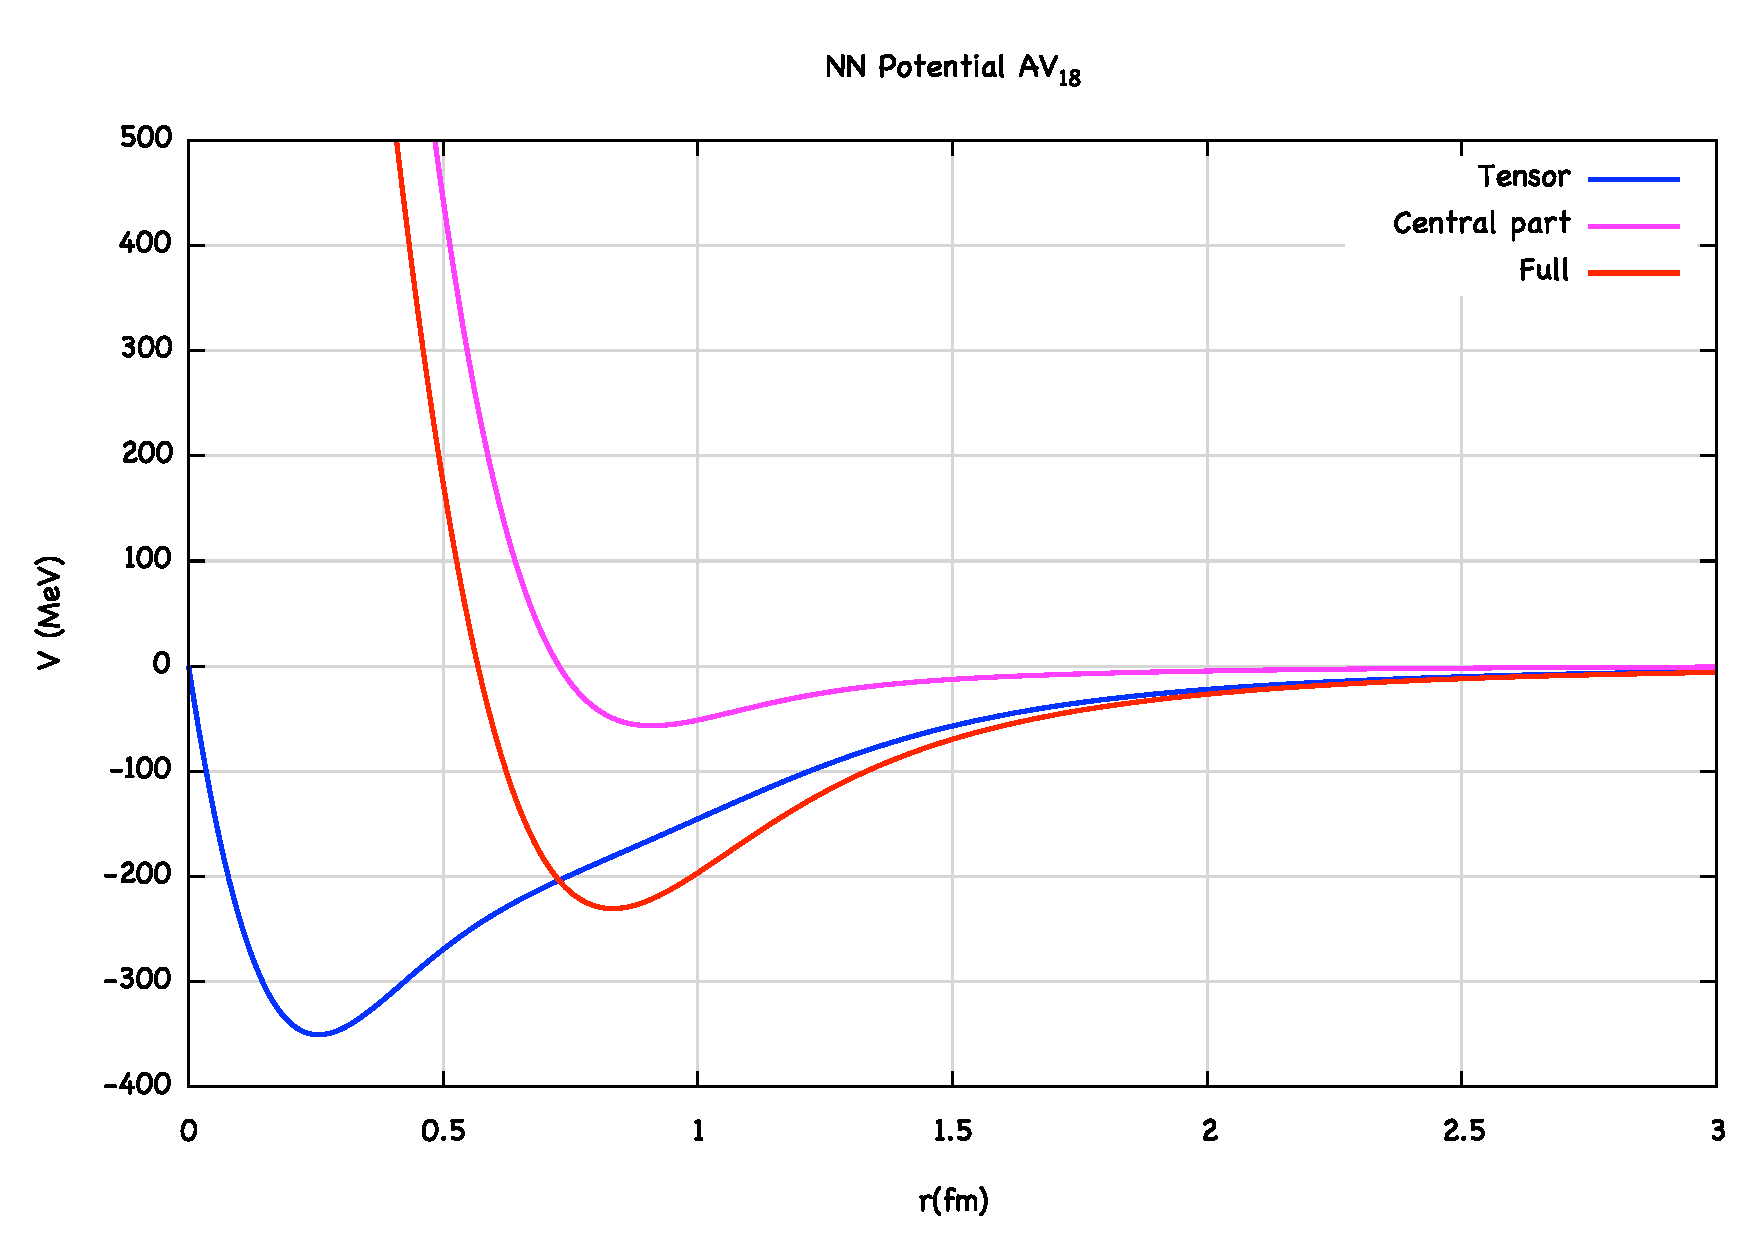
\includegraphics[type=pdf,ext=.pdf,read=.pdf,width=0.60\linewidth]{./figures/physics/CentralTensorFull}
    \caption[Two-nucleon potential distribution]{\footnotesize{Two-nucleon potential distribution \cite{donal_prvt}, where the blue line represents the tensor force which responds most of the attractive part.}}
    \label{potential_well}Compared with the general size of an atom, a
  \end{center}
\end{figure}

Furthermore, the particular behaviour of the interaction potential between nucleons also increases the complexity of the nuclear system. As shown in Fig.~\ref{potential_well}, two nucleons experience weak attractive interaction at moderate distance. As they get closer, the strong attractive force, mainly caused by the tensor components of spin and isospin channels, forms a deep potential well. At much short distance, the hard-core interaction between nucleons generates strong repulsion which prevents the nucleus from further collapses. The Coulomb force between protons and potential three-body forces also play a role but they are much weaker compared with the strong force.

Despite the complexity of the nucleus, Scattering experiment observed the spectroscopes of nucleons which reveal that nucleons behave more like independent particles in nuclear medium due to the collective effects of Pauli principle and the strong short-distant interactions with surrounding nucleons. Nucleons occupy different energy shells similar to the arrangement of electrons orbiting around the nucleus. 

The explanation of these phenomena has been successfully approached by independent particle shell model, in early circumstance also called as the mean field theory. In this theory, the nucleus is treated as a non-relativistic object where nucleons interact only through two-body interaction. Nucleons tend to occupy the lowest energy state first and the energy of the last occupied state is called the Fermi energy. The whole set of occupied energy levels is called the Fermi sea. Combined with the spin-orbit coupling, IPSM successfully predicts the ground state properties, the excitation of nuclei at low energy, nuclear spins and parities, as well as the prediction of nuclear magic numbers. However, IPSM shows its limitation in predicting the nuclear magnet moments and highly excited energy states. 
\begin{figure}[!ht]
  \begin{center}
    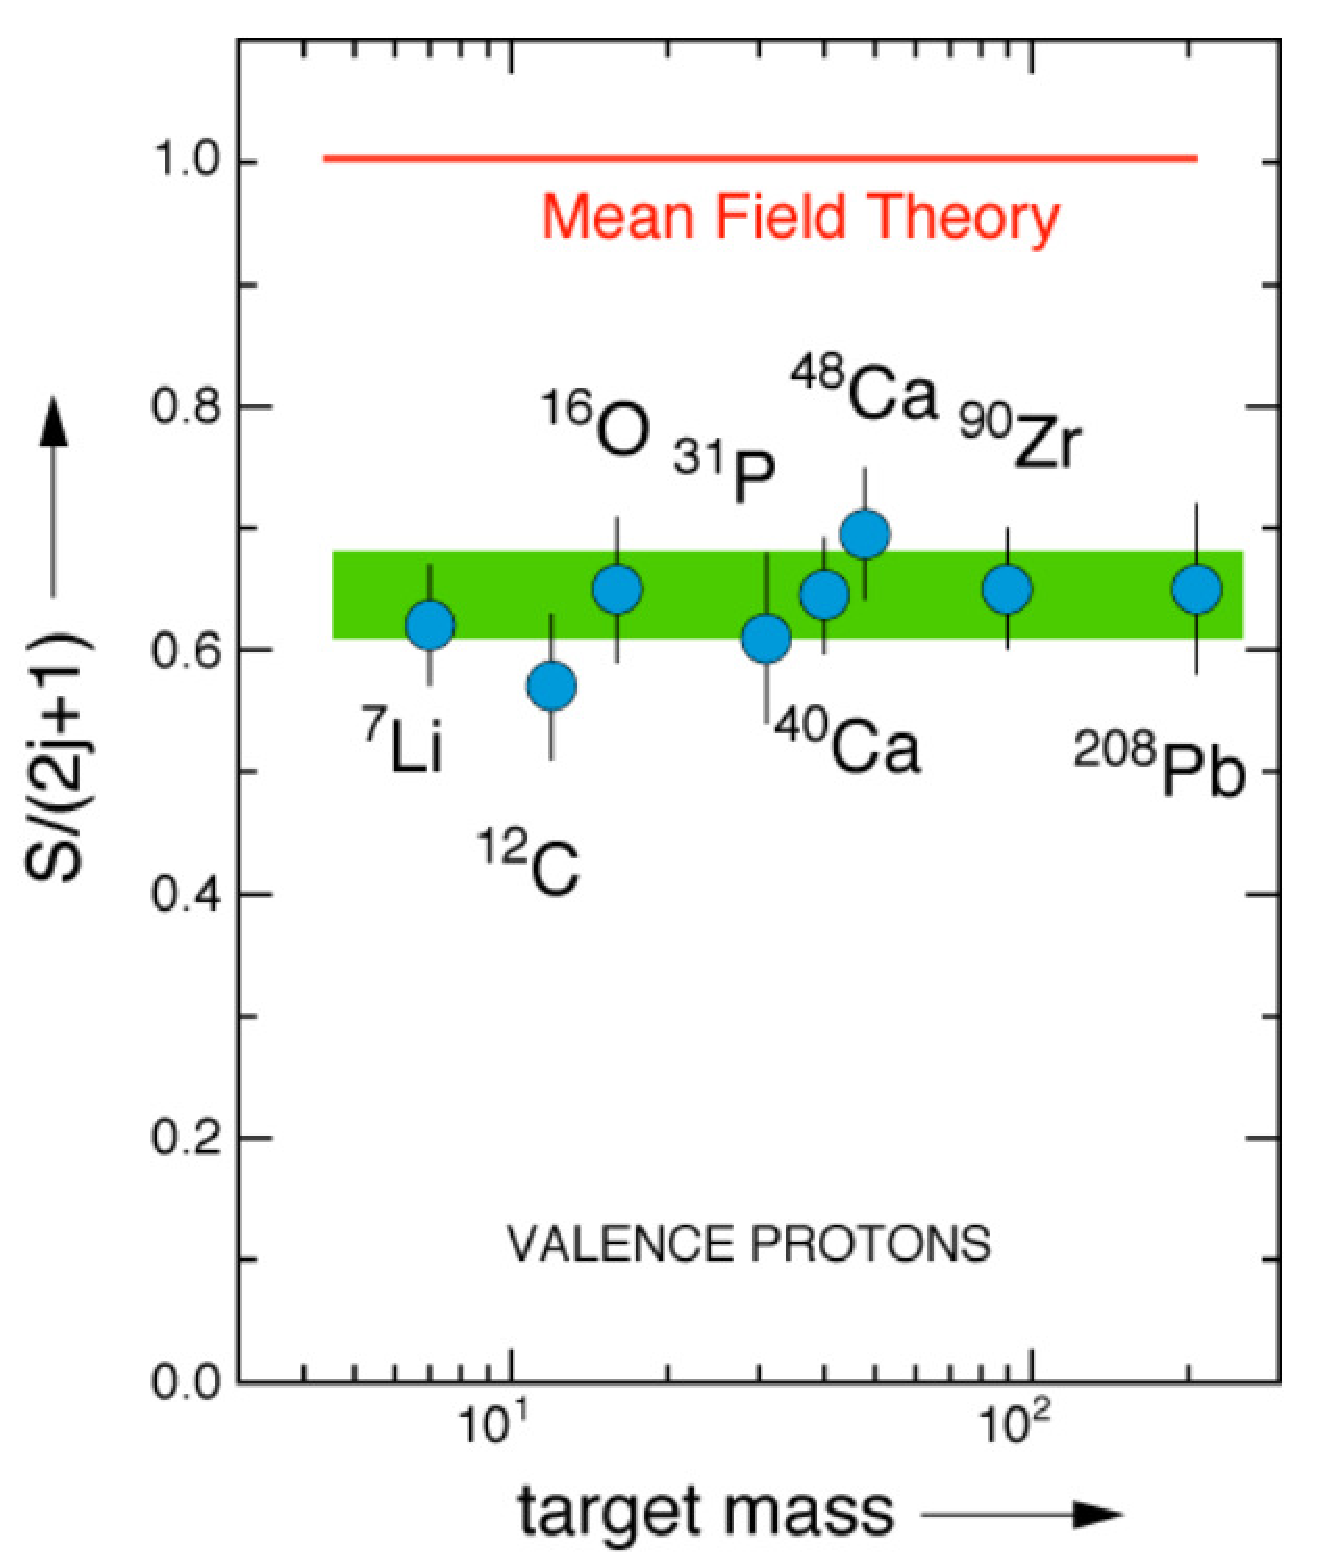
\includegraphics[type=pdf,ext=.pdf,read=.pdf,width=0.50\linewidth]{./figures/physics/spec_fac_exp}
    \caption[Experiment measurements of spectroscopy factors]{\footnotesize{Experiment measurements of spectroscopy factors for different nuclei deviate from one, indicating the important role of correlations between nucleons.}}
    \label{spec_fac_exp}
  \end{center}
\end{figure} 

A useful experimental observable, called Spectroscopy Factor, denotes the amplitudes of adding or removing one nucleon from the nucleus. In IPSM, assuming nucleons occupy $j$ orbits in the nuclear shell, the cross section of removing one nucleon is then written as, $\sigma_{removing} = S\cdot\sigma_{sp}$, where $\sigma_{sp}$ is the single-particle cross section, and the spectroscopy factor, $S$, should obey a sum role:
\begin{equation}
  \frac{S}{(2j+1)} \equiv 1,
\end{equation} 
where the factor $(2j+1)$ denotes the maximum energy states of the nucleon. Several measurements ~\cite{Lapikas1993297,Kelly:1996hd} with medium-energy proton-knock experiments in early 1970s measured the values of spectroscopy factor for heavy nuclei (Fig.~\ref{spec_fac_exp}) which is $30\%-40\%$ lower than one. Even advanced Hartree-Fock calculations~\cite{hartree_fock_book} involving long range nucleon-nucleon interaction still overestimate the nuclear strength.
